\documentclass[9pt,twocolumn]{article}
\usepackage[margin=0.65in,top=0.5in,bottom=0.5in]{geometry}
\usepackage{amsmath,amssymb}
\usepackage{graphicx}
\usepackage{booktabs}
\usepackage{enumitem}
\usepackage[small,compact]{titlesec}

\setlength{\parskip}{3pt}
\setlength{\parindent}{0pt}
\setlength{\dbltextfloatsep}{6pt}
\setlength{\dblfloatsep}{6pt}

\pagestyle{empty}

\begin{document}

\twocolumn[{%
\centering
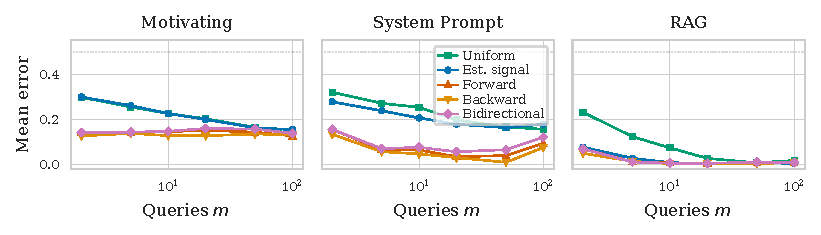
\includegraphics[width=0.88\textwidth]{figures/figure_query_selection_methods.pdf}

{\small\textbf{Figure 1.} Mean classification error vs.\ query budget $m$ for three selection strategies across three tasks ($n{=}80$). Stepwise selection matches uniform sampling accuracy with $5$--$10\times$ fewer queries.\par}
\vspace{1em}
}]

\section{Motivation}

Classifying black-box generative models requires querying each model and comparing responses via pairwise energy distances.
In a typical workflow, a labeled pilot set of $n$ models is queried on a large pool of $M$ queries, and the cached responses are used to estimate the discriminative structure.
The cost of classifying a \emph{new} model scales with the number of queries $m$ it must answer --- each query is an API call.
Identifying a small, high-quality query set $Q^*$ of size $m \ll M$ that preserves classification accuracy therefore directly reduces the per-model audit cost for all future models.

\section{Methods}

We consider three ways of selecting a query set for which we generate responses for each new model.

\textbf{1.\ Uniform Sampling} (baseline).
Sample $m$ queries uniformly at random from the pool of $M$ queries.
No pilot information is used.

\textbf{2.\ Estimated Signal Sampling.}
Fit a two-component GMM to the SVD loadings $|U_{q,\ell}|$ of the energy tensor $E$.
Queries assigned to the higher-mean component form the estimated signal set $\hat{\mathcal{S}}$.
Sample $m$ queries uniformly from $\hat{\mathcal{S}}$.
This exploits zero-set structure but ignores query redundancy.

\textbf{3.\ Forward Stepwise Selection.}
Define a response $z_{ij} = \mathbf{1}[y_i \neq y_j]$ for each model pair and a predictor $E_{q,ij} = \|g(f_i(q)) - g(f_j(q))\|^2$ for each query $q$.
At each step, add the query whose $E_{q,:}$ has the largest partial correlation with the residual of $z$ after projecting out previously selected queries.
This is Gram-Schmidt orthogonalization on $E$ w.r.t.\ $z$, ensuring each query contributes maximally non-redundant signal.
Cost: $O(m \cdot M \cdot \binom{n}{2})$ --- negligible.

\section{Setup}

\begin{table}[h]
\vspace{-0.5em}
\centering
\small
\begin{tabular}{@{}lccp{3.2cm}@{}}
\toprule
Task & $n$ & $M$ & Description \\
\midrule
Motivating & 100 & 200 & Sensitive training data \\
Sys.\ Prompt & 100 & 200 & Covert persuasion bias \\
RAG & 120 & 200 & Unauthorized doc.\ stores \\
\bottomrule
\end{tabular}
\vspace{-0.5em}
\end{table}

$n_{\text{train}} = 80$ models for estimation and classification; rest held out.
MDS (8 components) $+$ LDA. Averaged over 100 random splits.

\section{Results}

Stepwise dominates at small $m$: at $m{=}2$, stepwise error is $10\%$ (motivating) and $11\%$ (system prompt) vs.\ $28\%$ for uniform.
Estimated signal is intermediate, confirming the GMM partition captures real structure.
On the system prompt task, stepwise at $m{=}5$ matches uniform at $m{=}50$ --- a $10\times$ reduction in per-model query cost.

\end{document}
